\chapter{Departmental Context}

The Coffee Chain ERP system is designed to align organizational departments with structured digital workflows. By mapping operational units into a central platform, the ERP ensures clarity in roles, accountability, and information flow.

\section*{Departments Covered}
\begin{itemize}
    \item \textbf{Outlet Management:} Maintains details of each coffee outlet such as name, location, and management assignments. This ensures visibility of operational capacity across the chain.
    \item \textbf{Sales:} Records daily transactions, revenue, and order details in real time to support both operational monitoring and long-term planning.
    \item \textbf{Customer Relationship Management (CRM):} Tracks leads, customer details, and engagement history, enhancing marketing and customer retention.
    \item \textbf{Menu Management:} Provides a master list of products, categories, and pricing, synchronized with the sales process for consistent ordering.
\end{itemize}

\section*{Integration with QMS and PDCA}
The ERP modules operate under a quality-driven approach, embedding the PDCA (Plan-Do-Check-Act) cycle:

\begin{itemize}
    \item \textbf{Plan:} Departments define objectives such as increasing sales, improving customer engagement, or optimizing outlet operations.
    \item \textbf{Do:} Daily activities are executed through ERP modules, standardizing operations across outlets.
    \item \textbf{Check:} Performance indicators are tracked in reports and dashboards to measure actual outcomes against plans.
    \item \textbf{Act:} Managers adjust strategies, update menu items, or refine CRM tactics based on data-driven insights.
\end{itemize}

\section*{Interaction Diagram}
\begin{figure}[H]
\centering
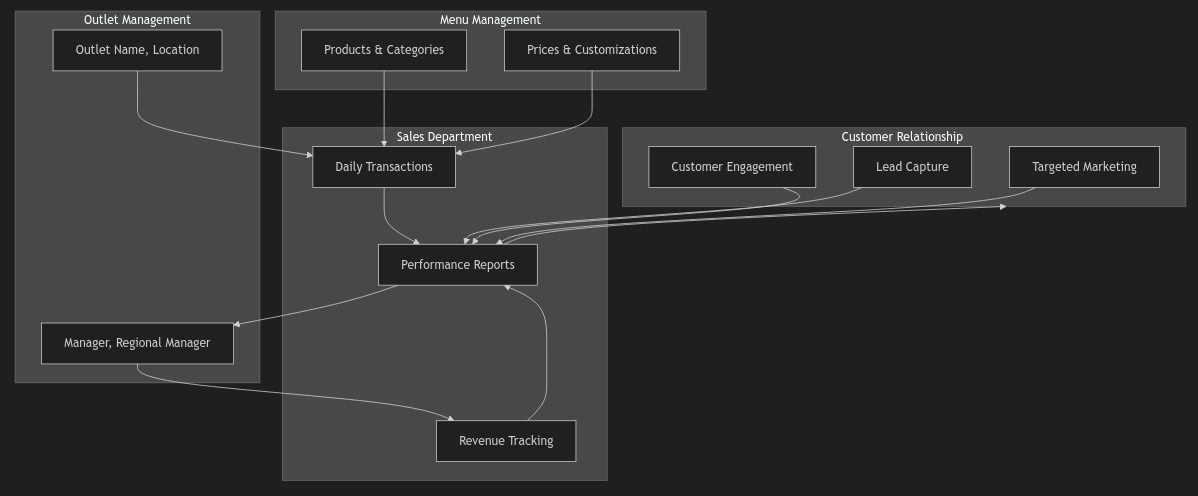
\includegraphics[width=0.9\textwidth,height=0.5\textheight,keepaspectratio]{diagrams/department.png}
\caption{Department Interaction Diagram of Coffee Chain ERP}
\end{figure}

\section*{Insights}
\begin{itemize}
    \item Departments are digitally connected, reducing fragmentation of data.  
    \item Centralization improves accuracy and ensures a single version of truth.  
    \item PDCA integration provides a cycle of continuous improvement.  
\end{itemize}
